%!TEX root = ../dissertation.tex
\section{Cholinergic Systems}
\newthought{Nary a process in the mammalian body can commence without participation of cholinergic systems.} \Ac{ach} was chemically and pharmacologically described by Henry Dale more than 100 years ago\cite{Dale1914}. A short time later, Otto Loewi published the first proof of signal transmission by small molecules: he transferred physiological solutions from electrically stimulated frog hearts to naive hearts and observed their reactions; the solution that provoked a parasympathetic response he proposed to contain a »vagus substance«\cite{Loewi1921}. Finally, in 1929, Henry Dale completed the picture by isolating acetylcholine from mammalian tissue and identifying it as the molecule responsible for the parasympathetic response\cite{Dale1929}. Dale and Loewi's joint effort in »Discoveries Relating to Chemical Transmission of Nerve Impulses« was rewarded with the »Nobel Prize in Physiology or Medicine« in 1936.

Although we have learned much about cholinergic systems in these past 100 years, our understanding of the mammalian nervous system still is fairly limited. Even when disregarding peripheral nervous systems, the complexity of cholinergic transmission is immense, and a myriad functions have been attributed to cholinergic circuits in the \ac{cns}. Central nervous projections of cholinergic fibres were extensively mapped by Marek-Marsel Mesulam and others in the 1980s\cite{Mesulam1984, Mesulam1988}, with a majority of long projection neurons originating in one of the eight cholinergic nuclei, Ch1-Ch8. While many of these anatomical structures have been filled with meaning by associations with both rudimentary as well as higher brain functions, there are still as many cholinergic pathways whose function is entirely unclear (Figure \ref{fig:projections}, from Lobentanzer \emph{et al.}\cite{Lobentanzer2019a}). This holds particularly true for the only recently discovered cortical cholinergic interneurons, which, in comparison to their projecting counterparts, are very small and numerically vastly inferior to other neuron types in the cortex. Thus, their detection and analysis with current methods is challenging. 

\begin{figure}
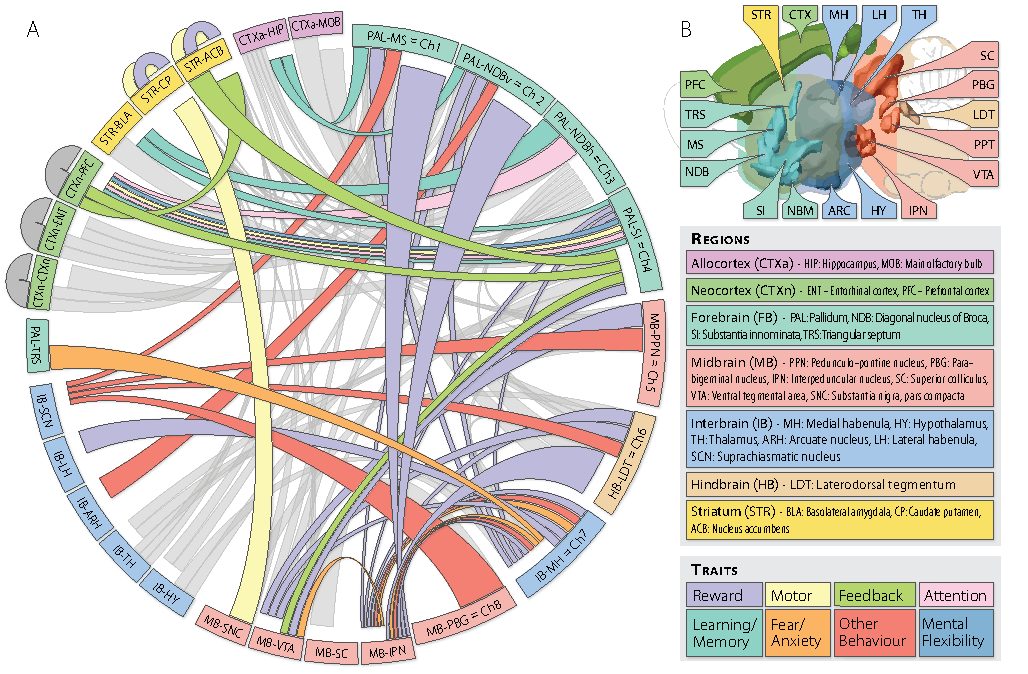
\includegraphics[width=\textwidth]{figures/projections}
\caption[Cholinergic Projections.]{\textbf{Cholinergic Projections in the CNS.} Cholinergic systems are implicated in many diverse functional categories. \textbf{A)} The bulk of cholinergic projection neurons stems from one of the eight cholinergic nuclei, Ch1-Ch8 (right side of ideogram). They innervate wide areas of the mammalian CNS, and in turn receive incoming connections from all around the brain (left side of ideogram). Efferent connections are indicated by a small gap between ideogram and connector, in the first clockwise half of each ideogram component, afferent connection by a large gap, in the second half. A number of projections has been associated with specific functions, as implicated by the colours of the connectors. Two populations of cholinergic interneurons have been identified, in the striatum and the neocortex (outside of ideogram). \textbf{B)} Brain region and trait colour legend for A).
\label{fig:projections}}
\end{figure}

The histological definition of what constitutes a cholinergic neuron is not without debate. The staining procedures established in the 1970s utilised monoclonal antibodies against \ac{achep}\cite{Mesulam1976}, whose association with cholinergic neurons is not definitive, as it can be expressed post-synaptically as well (for an overview of genes of the cholinergic systems, see Box \ref{box:chol-genes}). Later on, developments in horseradish peroxidase systems allowed immunohistochemistry on \ac{chatp}, which is a more immediate marker of cholinergic neurons\cite{Mesulam1984}, albeit much more lowly expressed than AChE. However, AChE-based staining still was consistently used in addition to ChAT staining\cite{Mesulam1988}, sometimes without much differentiation. Recently, single-cell \ac{seq} allows a more detailed appreciation of the transcriptional diversity of neurons, and enables a clearer distinction between cholinergic and non-cholinergic neurons expressing AChE (see Section \ref{sec:cellculture:singlecell}).

\begin{mybox}{The Cholinergic Genes}\label{box:chol-genes}
Acetylcholine is synthesised from acetyl-CoA - supplied by \textbf{ATP citrate lyase} (\emph{ACLY}) - and choline via enzymatic catalysis by \textbf{choline acetyltransferase} (ChAT from the \emph{CHAT} gene). It is then packed into vesicles by the \textbf{vesicular acetylcholine transporter} (vAChT from the \emph{SLC18A3} gene). After release into the synaptic cleft, it binds to a variety of \textbf{nicotinic and muscarinic receptors} (\emph{CHRNx}, 16 subunits, and \emph{CHRMx}, 5 subtypes). Of those, the nicotinic receptors form heteropentameric or, seldom, homopentameric ion channels, while the muscarinic receptors are monomeric G protein-coupled transmembrane receptors. The human possesses a duplicate of the nicotinic $\upalpha$7 receptor, \textbf{dup$\upalpha$7} (\emph{CHRFAM7A}), which cannot bind ACh and supposedly acts as a dominant negative regulator of the $\upalpha$7 homomeric receptor. Termination of the signal is mainly achieved by \textbf{acetylcholinesterase} (AChE from the \emph{ACHE} gene), one of the fastest enzymes known, with a theoretical rate of \num{25000} molecules per second. AChE tetramers are usually tethered to cell membranes in the synaptic vicinity by the \textbf{proline-rich membrane anchor} (\emph{PRIMA1}) or \textbf{collagen Q} (\emph{COLQ}) peptides. Complementary to the mostly residual AChE is the circulatory \textbf{butyryl cholinesterase} (BChE from the \emph{BCHE} gene), which can also nonspecifically degrade ACh. After degradation, residual choline is reimported into cells via the \textbf{high affinity choline uptake transporter} (HACU, from the \emph{SLC5A7} gene).
\end{mybox}

\section{Cholinergic Aspects of Disease} \label{sec:intro:diseases}
\newthought{Cholinergic systems are integral} for a myriad physiological functions, and as such they are critically involved in aetiologies and phenotypes of a number of central and peripheral diseases. Of interest to this dissertation are the cholinergic aspects of degenerative and non-degenerative central nervous diseases (such as Alzheimer's Disease, Bipolar Disorder, Schizophrenia), ischemic conditions in stroke, and peripheral modulation of immune responses, particularly in the context of the aforementioned diseases.

\subsection{Alzheimer's Disease}
\ac{ad} was characterised by Alois Alzheimer in 1906 and later named after him by his colleague and mentor, Emil Kraepelin\cite{Berrios1990}. AD is a progressive neurodegenerative disease, its main risk factor is age, and it is estimated to make up 60-70\% of all dementia cases. The disease incidence and progression distinctly differ between the sexes\cite{Miech2002}; generally, women are affected more often. Unlike the very rare familial form (that can affect patients in their fifties), spontaneous AD usually only begins to manifest symptomatically in the 6th to 7th life decade. As a result of the demographic change in most western countries, patient numbers, and thus, medical efforts, are expected to more than double in size until the year 2050. The cognitive decline associated with AD is progressive and ultimately leads to exhaustive care dependency; there is no cure.

The pathological hallmarks of AD are two types of atypical protein aggregates, inter-cellular amyloid $\upbeta$ »plaques«, and intra-cellular »neurofibrillary tangles« composed of hyper-phosphorylated tau-protein. Often, pathological aggregation of these proteins begins decades before the onset of symptoms. However, there have also been numerous cases of cognitively healthy subjects showing high amounts of protein aggregates. These inconsistencies and the unclear causality of pathology and symptoms have led to a redirection of scientific efforts to processes unrelated to amyloid and tau, such as neuroinflammation.

Cholinergic systems have long been associated with AD, as evidenced by the cholinergic hypothesis that was posed in the 1980s. To cite from Bartus \emph{et al.}, 1982\cite{Bartus1982}:

\begin{quote}
»We have been guided by three deductive requirements that must be satisfied if the cholinergic hypothesis is to deserve continued attention: (i) specific dysfunctions in cholinergic markers should be found in the brains of subjects suffering from age-related memory loss, (ii) artificial disruption of central cholinergic function in young subjects should induce behavioural impairments that mimic the cognitive loss found naturally in aged subjects, and (iii) appropriately enhancing central cholinergic activity in aged subjects should significantly reduce age-related cognitive deficits.«
\end{quote}

Although many reports substantiate all three deductive prerequisites, the cholinergic hypothesis has in the last decades been overshadowed by alternative hypotheses, particularly, amyloid-related theories. However, the therapeutic approaches developed along the lines of preventing amyloid $\upbeta$ aggregation or otherwise clearing the plaques or soluble aggregates have not been successful in alleviating the cognitive decline in patients(cite). Thus, pro-cholinergic intervention by means of \ac{achep} inhibition still makes up the majority of approved drugs. The monotherapeutic approach of AChE inhibition is based on a premise that seems simple in light of the enormous complexity surrounding the interplay of the billions of neurons in the process of memory formation and recall, and in fact, pro-cholinergic therapy has only been shown to alleviate symptoms or delay their onset; a reversal of cognitive losses has so far not been achieved by any drug regime. As such, even in regard only to the cholinergic systems, novel approaches are sorely needed.

On the other hand, the cholinergic deficit in AD is not purely symptomatic. There is considerable debate whether the pathology originates from the entorhinal cortex or the basal forebrain. As Heiko and Eva Braak have shown\cite{Braak1995}, AD pathology follows a characteristic brain region distribution process that can be stratified into stages and starts in the entorhinal region. The early stages of pathology by far precede the onset of symptoms. Taylor Schmitz and colleagues substantiate the cholinergic origin of neurodegeneration in their longitudinal \emph{in vivo} imaging studies\cite{Schmitz2016, Schmitz2018}: In cognitively normal and impaired human subjects, basal forebrain volume predicted longitudinal entorhinal degeneration, but not \emph{vice versa}. As such, the cholinergic basal forebrain dysfunction precedes as well as predicts pathology in other affected areas and cognitive deficits\cite{Schmitz2016}. Additionally, the spread of Alzheimer's pathology in the longitudinal progression of the disease reflects the spatial topography of basal forebrain cholinergic projections\cite{Schmitz2018}.

% sexual dimorphism in response to ache inhibitors Giacobini2018

%Li Gan - NFkB activation by tau
% - Ikkbeta knockout corrects STAT1 DE

\subsection{Schizophrenia and Bipolar Disorder} 
Cognitive deficits can also occur without neuron death. The earliest description of what we today call \ac{scz} was coined by Emil Kraepelin: »\emph{dementia praecox}«, premature dementia\cite{Kraepelin1913}. Cognitive deficits are an integral but often overlooked part of the clinical picture of SCZ, which is often dominated by the more impressive positive symptoms such as hallucinations and paranoia. Likewise, \ac{bd} can present with cognitive impairments. The cognitive impairments affecting both SCZ and BD patients involve diminished problem solving capabilities and reduced intelligence, and are more pronounced in SCZ than in BD\cite{Bortolato2015}. They have been connected to cholinergic dysfunction\cite{VanEnkhuizen2015, Smucny2017} and the sum of anticholinergic medications\cite{Gray2015, Eum2017}. A human polymorphism in the $\upalpha$5 nicotinic receptor subunit predicts a higher propensity for smoking and SCZ, showing parallel manifestations in engineered mice\cite{Koukouli2017} and rats\cite{Forget2018}. Correspondingly, cholinergic stimulation can improve cognition\cite{Sacco2004, Rowe2015, Lewis2017} and mood\cite{Higley2014}, but can on the other hand provoke schizotypic behaviour in AD patients\cite{Degirmenci2016}.

SCZ and BD clinically present with clear sexual dimorphisms. Compared to women, men have a higher SCZ prevalence with an \ac{or} of 1.4, are affected earlier (at 15-25 as compared to 25-35 years of age), and face a worse prognosis\cite{Leger2016}. Cholinergic participation also appears sex-dependent: Male SCZ patients more often self-medicate by smoking (7.2 versus 3.3 weighted average OR with 90\% lifetime prevalence)\cite{DeLeon2005}. BD, on the other hand, affects men and women almost equally, with an OR of $\smallsim$\num{1}. However, women make up 80-90\% of so-called »rapid cyclers«, a subgroup of patients showing short intervals between manic and depressive phases which is associated with a worse prognosis\cite{Berger2014}. Additionally, major depressive disorder, which is a prerequisite for BD diagnosis, more often affects women\cite{Berger2014} (OR = 2).

Psychiatric genomics has recently identified a high amount of shared heritability between SCZ and BD\cite{Anttila2018}. Likewise, transcriptomic analyses have shown a high correlation (71\%) between the transcriptional perturbations in the two diseases\cite{Gandal2018}. Clinical as well as molecular pathology intensifies from BD to SCZ, suggesting the two lie on different points of a shared spectrum. However, their genetic origins are tremendously complex. Multiple disease-relevant markers have been identified by GWAS (genome-wide association studies), even able to distinguish between several sub-phenotypes of each disease\cite{Ruderfer2018}. These markers are found in neurotransmitter receptors (e.g., dopaminergic, glutamatergic, cholinergic), scaffolding proteins (DISC: »disrupted in schizophrenia«), multiple \acp{tf}, \acp{mir}, and non-coding regions without known function\cite{Harrison2015, Henriksen2017, Kanazawa2017}.

Considering this complex disease aetiology, it is not surprising that there are no »designer« drugs available against SCZ and BD. All available therapeutic options have been empirically found, starting with the first antipsychotic, chlorpromazine, synthesised in 1950 by the French pharmaceutical company Rhône-Poulenc. Originally developed in a series dedicated to the search for antihistaminics, it was soon recognised for its antipsychotic potential, and widely prescribed only few years later. Many other neuroleptic compounds have been derived from chlorpromazine, and through binding affinity assays, their receptor profiles were established. Most compounds with antipsychotic properties have a wide spectrum of different receptor activities, but most early drugs were strong antagonists of the D$_2$ dopamine receptor. Thus, the »dopaminergic hypothesis« of SCZ was formulated. However, aetiology as well as therapeutic principles are unclear to this day, and most antipsychotic substances still are very »dirty drugs«. In fact, newer developments leading to the discovery of the second generation (»atypical«) neuroleptic substances, starting with clozapine, have created molecules with an even wider spectrum of interactions und thus less specificity towards a single therapeutic mechanism of action. Similarly, the archetypal »mood stabiliser« Lithium, that has been found to ameliorate depressive as well as manic phases of BD, likely influences a wide variety of neuronal functions via mechanisms yet unclear\cite{Malhi2013}. This general development is contrary to pharmaceutical research practice, where most developments aim for a higher specificity. It is thus very likely that pharmacological therapy of SCZ and BD requires an approach consisting of multiple pharmacodynamic angles, to account for the multigenic disruption.

\subsection{Immunity} \label{sec:intro:immunity}
Aside from its vast neuronal functions, \ac{ach} also is highly relevant in immune cells, recently reviewed by Fujii and colleagues\cite{Fujii2017}. The first to isolate ACh from an animal organ, Dale and Dudley\cite{Dale1929}, used the spleens of oxen and horses. The spleen receives sympathetic, but not parasympathetic innervation, and as such, the ACh found by Dale and Dudley had to have come from immune cells. Indeed, nearly all mammalian immune cells express cholinergic components, most importantly, B- and T-cells, macrophages, and dendritic cells. ACh is physico-chemically as well as enzymatically unstable, and thus has to be supplied synaptically or, at most, in paracrine fashion. Soluble esterases cleave ACh with stunning efficiency, reducing its diffusion range to few millimetres. \Ac{chatp} activity has been confirmed in B- and T-cells, which both contain significant amounts of ACh, although T-cells generally possess higher amounts. Additionally, in peripheral cells ACh can be synthesised by the mitochondrial carnitine acetyltransferase. In addition to B- and T-cells, \emph{\acs{chat}} mRNA has been found in macrophages and dendritic cells. \ac{chatp} expression and ACh synthesis can be induced by various immune mediators, such as \ac{lps} and \ac{tlr} agonists.

In addition to ACh synthesis, all of the aforementioned cell types can receive cholinergic signals. They express all muscarinic receptors as well as a selection of nicotinic receptor subunits, and the signal-terminating esterases. Although it is not completely clear how the parasympathetic signal reaches the immune cells, cholinergic activation as a result of inflammation can dampen the immune response in what is described as the »cholinergic anti-inflammatory reflex«\cite{Pavlov2017}. This reflex loop is designed to protect the body from pathogens and inflammation, but also from the harmful effects of immune stimulation. Upon afferent signalling through the afferent vagus nerve and humoral components, the brain releases humoral (via the hypothalamic-pituitary-adrenal axis) and neuronal (via the sympathetic and parasypathetic autonomous fibres) anti-inflammatory signals. The spleen has been identified as a pivotal organ in this response. Since none of the immune organs receives parasympathetic innervation, it has been proposed that the cholinergic activation is generated locally, with the help of sympathetic signalling to the organ\cite{Dantzer2018}.

A special role among cellular ACh receptors is occupied by the $\upalpha$7 nicotinic receptor subunit. Previously thought to exclusively form homopentameric ion-channel receptors, its functional characteristics have recently been extended. It has been found to form heteropentamers with $\upbeta$2 subunits, akin to the prominent $\upalpha$4$\upbeta$2 receptors in the brain, and an expression in immune cells also is likely. A hybrid duplication of the \emph{CHRNA7} gene with \emph{FAM7}, \emph{CHRFAM7A}, is translated to a functional protein (dup$\upalpha$7). However, it seems to lack ACh binding ability, and thus is thought to act as a dominant negative regulator of $\upalpha$7 receptor function. In addition to its ionotropic function, mainly by means of Ca$^{2+}$ transduction, the $\upalpha$7 receptor has been found to possess G-protein coupled metabotropic effects that can extend the duration of cholinergic activation. The $\upalpha$7 receptor can also, independently of Ca$^{2+}$, activate the JAK2/STAT3 pathway (see Section \ref{sec:intro:neurokine}) in macrophages, leading to suppression of \acs{nfkb} signalling.

On the other hand, cholinergic activation via M$_1$ and/or M$_5$ muscarinic receptors can lead to a positive immune response. The difference between muscarinic and nicotinic immune-signalling is elucidated by transgenic receptor \ac{ko} animals: Splenar cells from selective M$_1$/M$_5$-\ac{ko} mice secreted significantly lower amounts of the neuromodulators \ac{tnf}-$\upalpha$, \ac{ifn}-$\upgamma$, and \ac{il}-6 than those from \ac{wt} mice. Conversely, antigen-stimulated splenar cells from $\upalpha$7-\ac{ko} mice produced significantly greater amounts of \ac{tnf}-$\upalpha$, \ac{ifn}-$\upgamma$, and \ac{il}-6 than \ac{wt}. In summary, the effects of cholinergic stimulation of the immune system is bidirectional and strongly context-dependent, and specific pharmacological intervention can shift homeostasis in both pro- as well as anti-inflammatory directions.

\subsection{Neuroinflammation}
Neurodegenerative as well as non-degenerative neurologic diseases are increasingly being associated with immunologic phenomena, prompting the need for integrative and translational approaches\cite{Lurie2018}. Transient and chronic inflammatory events can influence neuronal function and even survival in a dramatic fashion. Further, failure to resolve the acute inflammatory states might lead to maladaptive states, cases of »frustrated resolution«\cite{Fullerton2016}, in which the goal of adaptive immunity is not met. As was recently shown\cite{Newson2014}, resolution of inflammation is not just the »phasing-out« of inflammatory events, but rather bridges the gap between innate and adaptive immunity. While many acute-phase T$_\mathrm{H}$1-type cytokines might have evolved to drive inflammation, their protracted influence may derail these post-inflammatory events and thus lead to maladaptive responses and chronic inflammation. T$_\mathrm{H}$1-type cytokines include \ac{tnf}, \acp{ifn}, IL-1$\upbeta$ and \ac{il}-6, and downstream mediators discussed in this context are manifold: \ac{pi3k}; \ac{camp}; \ac{mcl1}; the complex of \ac{bcl2}, \ac{akt}, and \ac{bad}; all variants of \ac{mapk}, i.e., \ac{erk} 1 and 2, \ac{jnk}, and p38 MAPK; and the \ac{nfkb} pathway. This list is not comprehensive, for a more detailed overview, see Fullerton \& Gilroy\cite{Fullerton2016}.

While none of the cardinal symptoms of inflammation are easily assessed in a \ac{cns} context, Vir"-chow's fifth cardinal sign, \emph{functio laesa}, is particularly difficult to tie to chronic neuroinflammation. Complex behavioural syndromes such as the functional deficits accompanying neurologic diseases might be influenced by protracted, maladaptive immunity, but the affected areas, brain structures, and timelines cannot be measured with current methods in neuroimaging. Only recently, it has become known that the brain is not immunologically pristine, but rather possesses a very specialised immune system, showing grave distinctions from, but also overlap with, peripheral immune systems\cite{Louveau2015, Negi2018}. The mechanisms of immune privilege of the brain are constantly being refined; there is crosstalk between brain and periphery with blood-to-brain and brain-to-blood messaging\cite{Dantzer2018}, and even migration of immune cells into the CNS, mainly as a response to sustained inflammation.

The first line of defence in CNS tissues are microglia, which in physiological state are resident ramified macrophages, and upon antigen sensing can produce an immediate native immune reaction. Further, the nascent immune system of the CNS comprises similar cells as the peripheral systems (T-cells, B-cells, NK-cells, dendritic cells), albeit with significant differences: antigen presenting cells express significantly fewer \ac{mhc} I and II molecules (which can however be induced by cytokine release upon inflammation); and the endocrine conditions (secretion of immune mediators from neurons) entail a more rapid response (seconds instead of days) with shorter duration of inflammation than in the periphery\cite{Negi2018}.

Under the surveillance of resident microglia, there is constitutive and inducible migration of immune cells between CNS tissues and periphery, in a loop of infiltration and drainage. Starting at antigen presentation inside the CNS, activated immune cells leave the CNS through one of two routes, both ending at the deep cervical lymph nodes: either through the cribiform plate into the nasal mucosa, or into the meningeal lymphatic vessels accompanying the sagittal and transversal sinuses in the \emph{dura mater}. Following an immunological stimulus, activated immune cells in the deep cervical lymph nodes facilitate a secondary immune response and protect nervous tissue through secretion of cytokines\cite{Walsh2015} and re-migration of secondary immune cells to the CNS. Regulatory cytokines include IL-1 and IL-6, CCLs and CXCLs, \ac{lif}, and epidermal and fibroblast growth factors. Re-migrating T cells can utilise various adhesion molecules expressed by endothelia along the blood-brain-barrier to cross into the CNS in a controlled fashion\cite{Negi2018}.

%Sabatino?\cite{Sabatino2019}

%The remarkable saga of the anti-inflammatory cholinergic reflex proposed by Kevin Tracey in the 2000s illustrates very well the various ingredients of the controversy about the parasympathetic innervation of lymphoid organs (171). The saga began with the discovery of unexpected pharmacological properties of a new anti-inflammatory drug developed by Tracey for the treatment of sepsis, tetravalent guanylhydrazone (CNI-1493). CNI-1493 was developed on the basis of its ability to inhibit the production of tumor necrosis factor-α (TNF) and other macrophage inflammatory cytokines in response to sepsis induced by administration of lipopolysaccharide (LPS). Tracey discovered that this lead compound was much more potent when injected into the lateral ventricle of the brain than when administered systemically (29). This finding was interpreted to indicate that CNI-1493 activates a neural pathway that links the brain to peripheral macrophages. This neural pathway was claimed to be the vagus nerves, as cutting the vagus nerves abrogated the anti-inflammatory activity of CNI-1493, whereas electrically stimulating the peripheral end of vagal nerves mimicked it (30).

%Indifferent to the controversies surrounding the possible existence of a parasympathetic innervation of lymphoid organs, Tracey (231) proposed that cholinergic vagal nerves act on macrophages to suppress the production of TNF and other inflammatory mediators. This neural communication pathway from the central nervous system to the immune system was presented as being part of an anti-inflammatory reflex whose afferent arm was the production of inflammatory cytokines by activated innate immune cells (see sect. III) and whose efferent arm was the activation of cholinergic efferents downregulating cytokine production by innate immune cells (FIGURE 1). Muscarinic cholinergic stimulation was proposed to mediate the central component of the anti-inflammatory pathway, whereas activation of nicotinic receptors containing an α7 receptor subunit mediated the downregulatory effect of acetylcholine on macrophages (242). What was still lacking in the characterization of this anti-inflammatory pathway, however, was an anatomically characterized target for the efferent vagal innervation (137).

\subsection{Stroke} \label{sec:intro:stroke}
Stroke is a medical emergency in which reduced blood flow leads to massive neuron death in the brain. There are two types of stroke: Haemorrhagic stroke, which is caused by bleeding due to a rupture of brain vessels, and ischemic stroke, misperfusion of a brain region caused by a clot in a cranial artery. Ischemic stroke makes up the vast majority of all strokes, about 90\%. Stroke is currently the second most frequent cause of death in developed countries, only second to coronary artery disease. Those who survive the stroke are in many cases permanently and severely disabled. The prognosis of stroke patients is mainly dependent on clinical complications during initial care.

Infections are a leading cause of death in stroke patients, the \ac{cns} injury itself is an independent risk factor for the development of life-threatening infection. The most frequent complications accompanying stroke are fever and pneumonia, the fever in turn being most often caused by the infection. Affecting more than 20\% of stroke patients, pneumonia is the most common serious post-stroke complication, featuring a mortality rate of more than 30\%\cite{Meisel2005}. Stroke patients demonstrate a significant immunosuppression, resulting in lower count and functionality of immune cells. The ability of monocytes to synthesise cytokines is drastically reduced, a finding that has been reproduced in animal models of cerebral ischemia.

T cell activation and proliferation in the deep cervical lymph nodes is elevated following CNS injury, implicating that the drainage of immune cells from the site of injury plays an important role in immune system stimulation\cite{Walsh2015}. Depletion of those T cell leads to neuron death, suggesting that this naive response is favourable in stroke and similar conditions. However, the specifics of activation and migration, and the mediators (cytokines, antibodies) influencing the post-injurious response are still largely unclear\cite{Louveau2015}.

The immunological situation after stroke is dominated by two opposing factors, the pro-inflam"-ma"-to"-ry bodily response to injury and, often, infection, and the counter-regulatory immunodepressive response including the cholinergic anti-inflammatory reflex (see Section \ref{sec:intro:immunity}). The inflammatory response can become pathologic in the case of excess stimulation, which can result in »systemic inflammatory response syndrome« (SIRS), which in extreme cases can lead to shock and organ failure. As a counterbalancing measure, the body responds with a »compensatory anti-inflammatory response syndrome« (CARS), designed to allow fighting the infection while also protecting the body from excessive immune stimulation. However, in \ac{cns} injury, the anti-inflammatory component might overwhelm inflammatory processes, leading to a pathological »CNS injury-induced immunodepression syndrome«, CIDS.

In addition to the humoral and neurohumoral immunomodulatory pathways described above, the brain can directly steer immune processes by the release of cytokines. This might be particularly impactful in CNS injury, where blood-brain-barrier and homeostasis are disrupted. Contrary to the selective uptake of substances into the CNS, export from the CNS is mostly instantaneous and not tightly controlled. Among the cytokines found in circulation after stroke are \ac{tgf}-$\upbeta$, IL-1$\upbeta$, \ac{il}-6, and \ac{tnf}-$\upalpha$. So far, it is unclear which of the immunomodulatory axes (humoral, neurohumoral, or direct release of cytokines from the brain) contributes to CIDS, and how they relate to each other. As a consequence, it is also unclear if directed intervention against CIDS would be beneficial, or even feasible\cite{Meisel2005}.

\subsection{Circadian Aspects of Cholinergic Systems}
Cholinergic systems and psychiatric diseases share another common theme: regulation of circadian time and sleep patterns. Cholinergic nuclei have been associated with the resetting of the circadian clock in the \ac{scn}. Retrograde tracing from the SCN\cite{Bina1993} has identified basal forebrain nuclei (Ch1 \& Ch4), as well as the pedunculo-ponitine nucleus (\acs{ppn}, Ch5), laterodorsal tegmentum (\acs{ldt}, Ch6), and the parabigeminal nucleus (\ac{pbg}, Ch8) as regulatory input to the SCN (compare also Figure \ref{fig:projections}). Basal forebrain cholinergic neurons are active in wakefulness and in the \ac{rem} phase of sleep\cite{Xu2015}, and optogenetic activation of PPN and LDT cholinergic neurons (channelrhodopsin 2 under the ChAT promoter) during non-REM sleep was sufficient to induce REM sleep in mice\cite{VanDort2015}. Basal forebrain projections to other brain regions seem to functionally diverge from the projections to the SNC. In a study analysing prefrontal and hippocampal cholinergic activities, the increase in tonic ACh release during REM sleep was contingent on subsequent wakefulness\cite{Teles-GriloRuivo2017}, and thus might convey a stronger »wake-up« signal than projections to the SCN alone.

Muscarinic receptors M1 and M3 are essential for REM sleep: REM-sleep is completely abolished in combined M1/M3 receptor \ac{ko} mice\cite{Niwa2018}. Arousal-induced phase shifts induced by activation of Ch4 cholinergic neurons projecting to the SCN were blocked in animals pretreated with (anti-muscarinergic) atropine injections to the SCN, demonstrating that cholinergic activity at muscarinic receptors in the SCN is necessary for arousal-induced phase shifting\cite{Yamakawa2016}. However, in their atropine perfusion experiment (locally via injection), the authors did not preclude cholinergic influences from the other nuclei. 

In parallel, psychiatric diseases regularly exhibit symptoms of disturbed circadian rhythm. In the cho"-li"-ner"-gic-catecholaminergic imbalance hypothesis of BD\cite{VanEnkhuizen2015}, the imbalance follows variable transcriptionally regulated rhythms, and affected individuals exhibit decreased \ac{rem} latency (the duration from onset of sleep to the first REM phase), which can be modulated by muscarinic agonists/antagonists\cite{Ising2005}. Conversely, sleep deprivation exerts short-term antidepressant effects \cite{Wu1990}, reduced cortical ACh levels\cite{Boonstra2007}, and vast transcriptional changes in basal forebrain cholinergic neurons\cite{Nikonova2017}.

While the \ac{scn} regulates circadian timing of the organism, individual cellular timings are controlled by a group of transcriptional activators and de-activators, called clock genes. The autoregulatory feedback loop thus created oscillates between day and night timing, under the influence of external factors. How exactly the individual cellular clocks are synchronised by the SCN is still unclear\cite{Balsalobre2002}. The first molecular circadian controller, \ac{clock}, was identified by Joseph Takahashi and colleagues via mutagenesis screening in mice in 1997\cite{King1997}. The transcription factors CLOCK and \ac{bmal} form heterodimers and bind to E-box elements in the promoters of \ac{per} 1 and 2, and \ac{cry} 1 and 2, which lead to negative feedback regulation; or to E-box elements in the promoters of \acs{nr1d1} (giving rise to the Rev-Erb$\upalpha$ protein) and \acs{nr1f1} (giving rise to ROR$\upalpha$), which compete for the ROR element in the \ac{bmal} promoter. ROR$\upalpha$ induces BMAL1 expression, while Rev-Erb$\upalpha$ represses it, thus leading to an oscillating expression pattern. In neurons, CLOCK can be substituted by its paralogue \acs{npas}.

\subsection{Neurokines} \label{sec:intro:neurokine}
In comparison to the widely studied cholinergic projection neurons originating in the basal forebrain (Ch1-Ch4) that are known to depend on a retrograde survival signal by means of \ac{ngf}, trophic influences on other cholinergic populations such as the cortical interneurons are unclear.  \ac{ngf} was described by Rita Levi-Montalcini in the 1950s as the first known instance of trophic peptides required for the survival of sympathetic ganglia\cite{Levi-Montalcini1960}. The group of neurotrophic substances since discovered (most prominently, the brain-derived neurotrophic factor \acs{bdnf}) are commonly referred to as »neurotrophins«. They convey their trophic effects through a family of transmembrane receptors; NGF binds to \ac{ntrk1} with high affinity, BDNF binds to \ac{ntrk2} with high affinity. However, both also bind to a third receptor, \ac{ngfr}, which is also known as p75, although with low affinity. NGFR function is complex, depending on the context it seems to be able to suppress as well as enhance the primary neurotrophic signal mediated by NTRK1/2(cite). The dependence of basal forebrain cholinergic neurons on retrograde NGF signalling was discovered in the 1980s\cite{Hefti1986}.  

A second group of trophic peptides with cholinergic implications are the so-called »neurokines«; the name results from the fact that this particular subgroup of cytokines has been associated with neuronal function in the central and peripheral nervous systems. Most prominently, they include the \ac{cntf}, \ac{lif}, and \ac{il}-6, all of which coincidentally have been known by the acronym CDF. In the late 1980s, two groups of scientists (McManaman\cite{McManaman1988} and Rao\cite{Rao1992}) independently identified proteins in extracts of muscle fibre that induced a differentiation of neurons towards a cholinergic type, and thus termed these proteins »choline acetyltransferase development factor« or »cholinergic differentiation factor« (both abbreviated CDF). Only later, through sequencing of the peptides, it became known that they had in fact discovered two distinct neurokines, \ac{lif} (Rao) and \ac{cntf} (McManaman, personal communication). \ac{il}-6, on the other hand, is abbreviated CDF for an entirely different reason: in this case it is short for »CTL (cytolytic T lymphocyte) differentiation factor«.

\ac{cntf}, \ac{lif}, and \ac{il}-6 convey their impact on neuronal activity through a partly redundant neurokine receptor pathway\cite{Berger2014}. There are two basic types of neurokine receptors: soluble and transmembrane. The primary receptors for \ac{cntf} (\acs{cntfr}) and \ac{il}-6 (\acs{ilr}) are soluble proteins that are secreted into the extracellular space and, upon binding of a neurokine, bind to transmembrane receptor dimers on the cell surface. These transmembrane receptors are the LIF receptor (\acs{lifr}) and the »interleukin 6 signal transducer« (\acs{ilst}, also known as \acs{gp}). Every neurokine has its preferred constellation of soluble and transmembrane receptors: \ac{cntf} binds to the soluble \ac{cntf} receptor and a dimer consisting of one \ac{gp} and one \ac{lifr} protein; \ac{il}-6 binds to the soluble IL6R and a dimer of two units of \ac{gp}; \ac{lif} does not usually bind a soluble receptor but rather binds immediately to a dimer comprising one of each \ac{gp} and \ac{lifr}; however, there is significant redundancy and crosstalk between those systems\cite{Rawlings2004,Nathanson2012}.

All receptor constellations result in a main effect of activation of the \acs{jak}/\acs{stat} cascade (Fig.\,\ref{fig:neurokine})\todo{remove miRs to later?}. More specifically, neurokines can activate \acfp{jak} 1 and 2 or the homologous \ac{tyk} 2, and, successively, \ac{stat} (»signal transducer and activator of transcription«) isoforms 1, 3, 5A, and 5B, which then convey a multitude of cellular effects (e.g. in immunity or differentiation) through transcriptional activation. The \ac{stat} cascade is inherently self-limiting in that it usually leads to expression of transcription factors that serve as repressors of the \ac{stat} genes by SOCS (suppressors of cytokine signalling), PIAS (protein inhibitors of activated STATs), and PTPs (protein tyrosine phosphatases)\cite{Rawlings2004}. 

Neurokines, particularly \ac{il}-6, might serve as a link between the immunological and cholinergic aspects of physiological or disease processes. Since IL-6 is implicated in neurodegenerative, psychiatric, and injurious CNS diseases (Section \ref{sec:intro:diseases}), which all also possess a cholinergic facet, it makes sense to not only see it in the light of an immunomodulator, but also as a potential influence on neuronal function in cholinergic systems. For instance, sleep disturbance in animal models of mood disorders is accompanied by elevation in blood levels of \ac{il}-1, \ac{il}-6, and \ac{tnf}-$\upalpha$\cite{Hodes2015}. Additionally, it has been shown that LIF can lead to a catecholaminergic-to-cholinergic neurotransmitter switch in peripheral neurons in a mouse model of protracted inflammation accompanying collagen-induced arthritis\cite{Stangl2015}. Though being a marginal phenomenon, it is not unthinkable that similar processes in central nervous cell might contribute to a disruption of homeostasis of cholinergic systems, and thus, to disease.

%from dantzer 2018: Another factor of confusion in the identification of cholinergic innervation of lymphoid organs is the existence of a catecholaminergic-to-cholinergic transmission switch in some sympathetic fibers influenced by signals, such as leukemia inhibitory factor, produced by the innervated target. Although this is a marginal phenomenon, it has been described in particular for the sympathetic fibers that innervate sweat glands in mammalian footpads (69) and the periosteum (6). Because the density of catecholaminergic neurons that innervate inflamed tissue decreases in patients with rheumatoid arthritis, the possibility of a catecholamine-to-cholinergic transition of sympathetic nerve fibers was investigated in a murine model of collagen-induced arthritis. Cholinergic sympathetic fibers became apparent several weeks after the induction of arthritis under the influence of leukemia inhibitory factor. However, catecholaminergic-to-cholinergic transition only affected those fibers that innervate healthy tissue adjacent to the inflammatory tissue (217). 

\begin{figure}
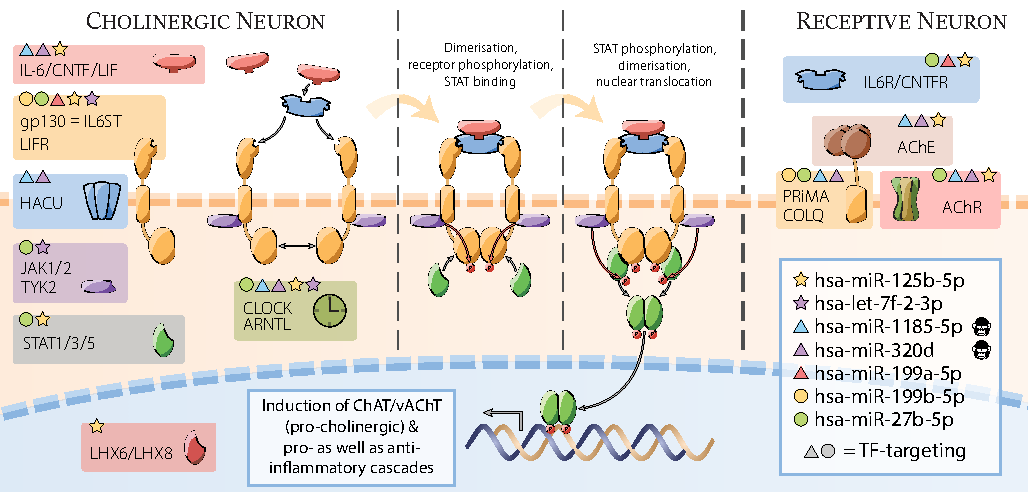
\includegraphics[width=\textwidth]{figures/neurokine}
\caption[The Neurokine Pathway.]{\textbf{The Neurokine Pathway.} The neurokines, such as CNTF, LIF, and IL-6, signal through a combination of soluble and membrane-bound receptors. Activation of a transmembrane neurokine receptor is usually followed by JAK recruitment and phosphorylation, and successively by STAT activation and translocation to the nucleus. Gp130-family neurokine, cholinergic, and circadian signalling pathways are controlled by primate-specific and evolutionarily conserved miRNAs. miRNA targeting of individual genes (indicated by coloured symbols) yields complex transcriptional interactions. Several miRNAs directly targeting the cholinergic pathway also target TFs controlling this pathway (circles and triangles).
\label{fig:neurokine}}
\end{figure}

%Neuronal activity is profoundly modified by cytokines

%Oleg Butovsky - TGFbeta as master glia regulator